\chapter{Technical Report}
\section{Introduction}
\subsection{Problem}
The subject of cybersecurity is constantly growing in importance for the computer scientist in general. The demand for cybersecurity experts with broad knowledge regarding current problems and malware is ever growing \cite{cybercrime-mag}. The Ostschweizer Fachhochschule (OST) has recognized this demand and has added more and more lectures for the cybersecurity interested students \cite{ost-cybersec}. One important aspect is still missing in the curriculum: reverse engineering.

\subsection{Similar Work}
To this date there is no work done regarding this subject in past projects. In the past, students have created different labs for the OST but none for reverse engineering. The infrastructure which is used for this project is already existing and established in the OST lectures. Hacking-Lab as the platform is known by the targeted student group and teachers alike. 

\subsection{Technologies Used}
To create each of the labs and their documentation multiple different tools and languages were used (shown in table \ref{tab:languages} and \ref{tab:tools}). 
\begin{center}
    \begin{table}[H]
        \centering
        \begin{tabular}{ |p{4.1cm}|p{10cm}| } 
            \hline
            \multicolumn{2}{||c||}{\textbf{Languages}} \\
            \hline
            \hline
                Assembler & As the base structure of a binary it was taught in multiple Courses before this. In the labs ASM is used to understand the flow of a function and what it does when executed. \\
            \hline
                C & All of the binaries were written in C.   \\
            \hline
                Python & As an easy to understand language Python is used to write the exploits after analyzing the binaries. \\
            \hline
        \end{tabular}
        \caption{Overview of all the languages used to create the labs.}
        \label{tab:languages}
    \end{table}
\end{center}

\begin{center}
    \begin{table}[H]
        \centering
        \begin{tabular}{ |p{4.1cm}|p{10cm}| } 
            \hline
            \multicolumn{2}{||c||}{\textbf{Tools}} \\
            \hline
            \hline
                VSCode & Each of the students of the project used VSCode for programming and documenting. This allowed for easier settings and more control of the output. \\
            \hline
                IDA Freeware & Each of the labs were tested before uploading to Hacking Lab. All of the tests were done in IDA Freeware since this software is used to show the solutions.  \\
            \hline
                Ghidra & Each of the labs were tested before uploading to Hacking Lab. Ghidra was used to check the pseudo code. This ensured that students using Ghidra instead of IDA Freeware have a solvable problem aswell and can follow the steps given. \\
            \hline
                HL Demo Tenant & 
                To test all of the labs, the demo tenant of Hacking Lab was used. This allowed for free testing without interfering with the OST tenant.  \\ 
            \hline
                Docker & Docker container can be used on the Hacking Lab platform to have a server side component to the challenges. \\
            \hline
                OST Gitlab & 
                To have versioning of the code OSTs Gitlab was used.  \\ 
            \hline
                Clockify & 
                This software allowed for time management. \\ 
            \hline
        \end{tabular}
        \caption{Overview of all the frameworks and tools used to create the labs.}
        \label{tab:tools}
    \end{table}
\end{center}

\subsection{Goals}
The goal for this project has multiple facets:
\begin{itemize}
    \item The creation of different labs to show the students of the OST the aspects of reverse engineering
    \item The students should have the following learning objectives:
    \begin{itemize}
        \item Gain an understanding of what reverse engineering is and what it can be used for
        \item Know the basic handling of debuggers and dissasemblers
        \item Understand a binary programs control flow using static debugging
        \item Understand a binary programs control flow using dynamic debugging
        \item Be able to locate and exploit simple security flaws in a binary program.
    \end{itemize}
\end{itemize}

\subsection{Product}
Since every student uses his own machine with his own configurations, Hacking-Lab as a platform with its LiveCD was chosen as foundation. This allows a simple, operating system independent approach to all excercises thanks to its webinterface and docker hosting capabilities. 

\section{Requirements for the Labs}

\subsection{Overview}
This chapter lists the different requirements we have defined in order to successfully create and solve the reverse engineering labs.
\subsection{Requirements}
\textbf{Language} \\
The labs and their solutions will be written in english to guarantee each student can understand it. \\[0.5cm]
\textbf{Targeted Group of Students} \\
The product of this project is aimed at students in their third year (fifth semester) or higher because it is an in-depth look at a cybersecurity subject. Students taking this course should have visited the mandatory subject "Cyber Security" to have basic information and maybe even "Secure Software" for more advanced knowledge of some exploitations. A rule of thumb is the more security lectures a student has visited and finished, the better. \\[0.5cm]
\textbf{Timerequirements} \\
Each of the labs has a different time requirement for the students. One lab should be solvable in an hour or less.  \\[0.5cm]
\textbf{Grading} \\
Depending on the lab, a student has to hand-in a flag, a writeup or a solved multiple choice. These will be checked by the teacher or an automated system. \\[0.5cm]

\newpage
\section{Lab Documentation}
% ------------------------------------------ INTRODUCTIONS ------------------------------------------ %
\subsection{Tools Introduction: GDB}
\subsubsection*{Problem Domain}
This lab covers the following aspects of the reverse engineering problem domain created by us:
\vspace{-2ex}
\begin{figure}[H]
    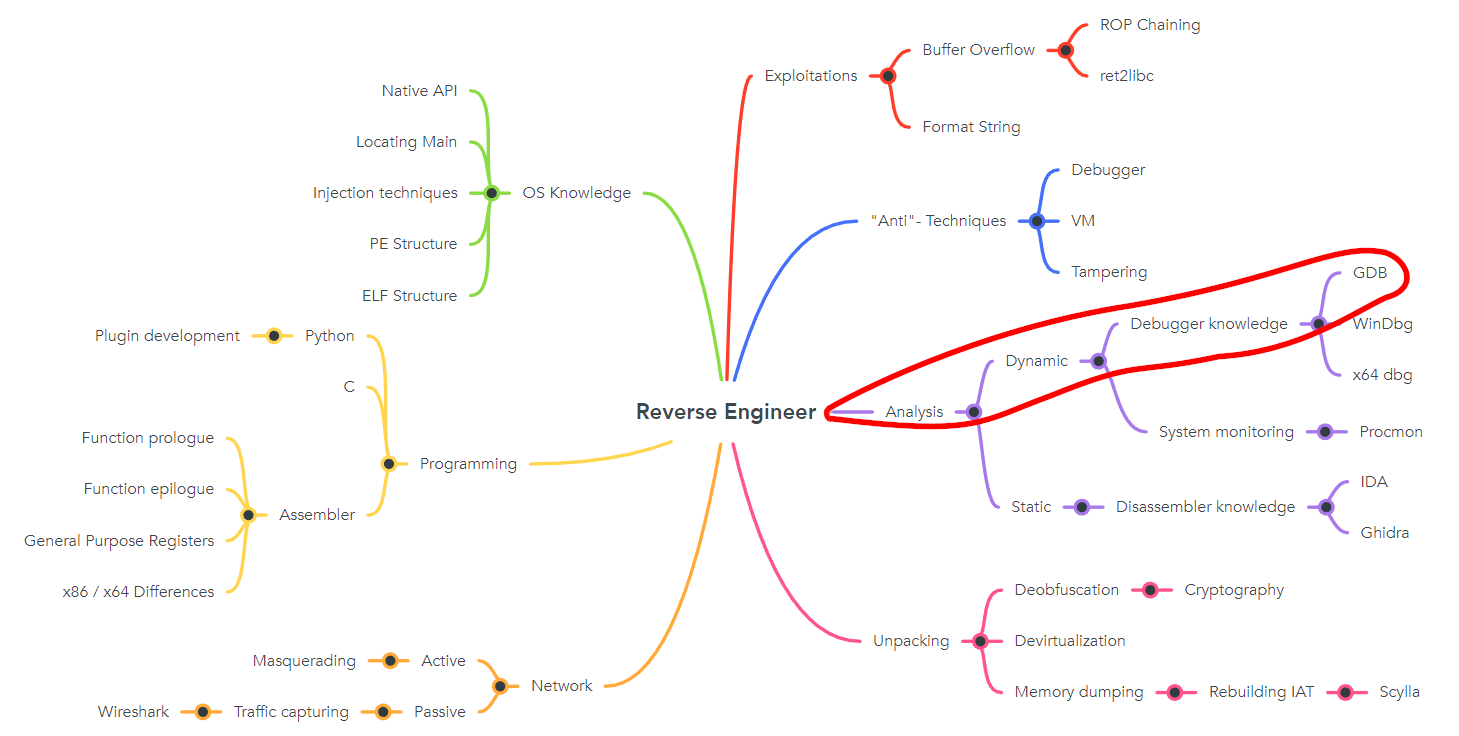
\includegraphics[width=\textwidth]{resources/GDBIntro-overview-light.png}
    \caption{GDB domain overview}
    \label{fig:gdb-overview}
\end{figure}
\subsubsection*{Content}
This introduction is used to explain the basic functionalities of the tool used in some of the labs. In this case GDB (GNU Debugger).
\subsubsection*{Choice of Topic}
The solutions and tips in the labs are given via screenshots or explanations. If a student wants to use a different tool he / she is free to do so. It is important that the tools used in the example solutions are known to the students. This makes it easier for them to understand each step and, if they are stuck at any point, follow the intructions on how to solve it. 
\subsubsection*{Objectives}
\begin{itemize}
    \item Learn about GDB and how to use the different commands available
\end{itemize}
\subsubsection*{Grading}
The labs are not graded since they are only used as a lookup. They have a flag to make sure the students have read the tools.
\pagebreak

\subsection{Tools Introduction: x64dbg}
\subsubsection*{Problem Domain}
This lab covers the following aspects of the reverse engineering problem domain created by us:
\vspace{-2ex}
\begin{figure}[H]
    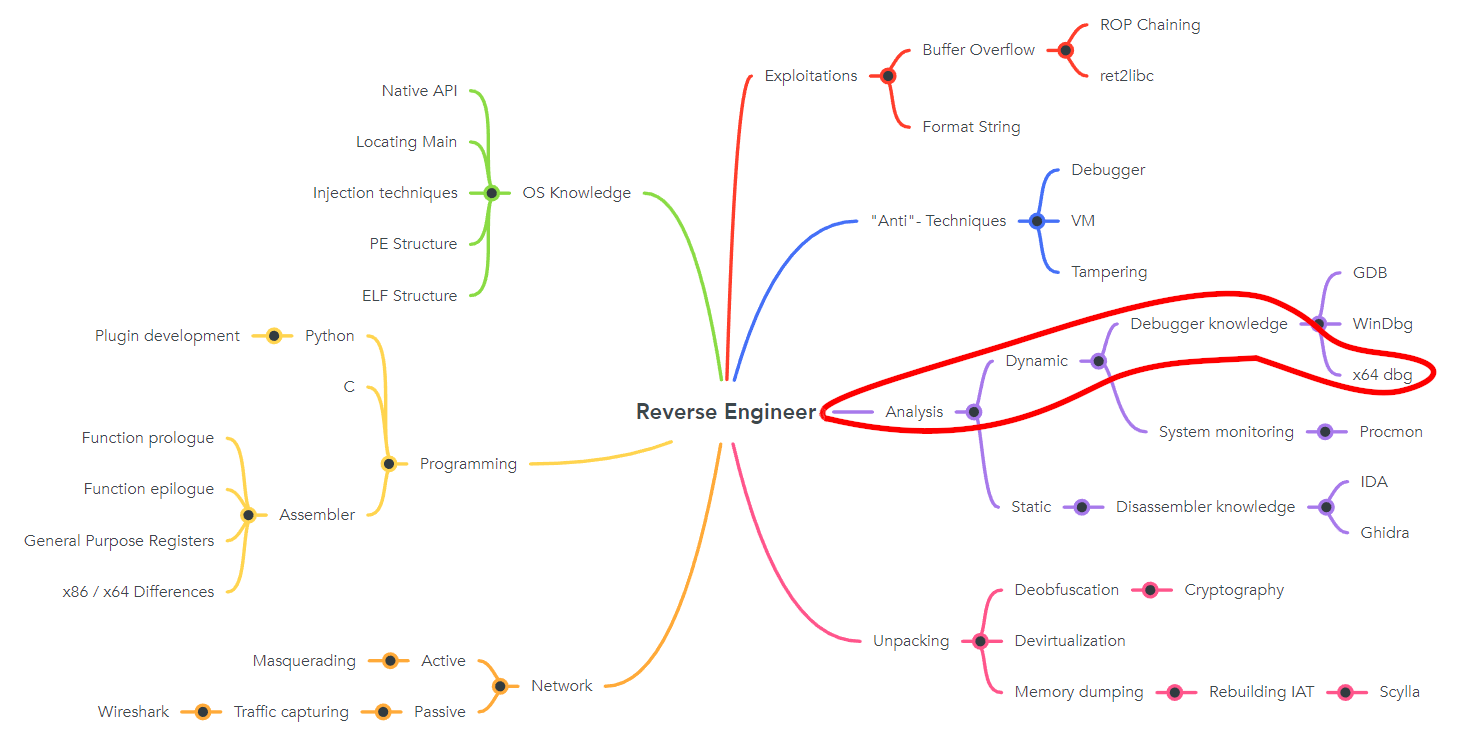
\includegraphics[width=\textwidth]{resources/x64Intro-overview-light.png}
    \caption{x64Intro domain overview}
    \label{fig:x64Intro-overview}
\end{figure}
\subsubsection*{Content}
Because most students have probably never touched a debugger on Windows before, this lab will help getting their feet wet with one of the most widely used ones by professionals.
This lab also acts as the basis for the upcoming labs where x64dbg will be used.
\subsubsection*{Choice of Topic}
Students working with Windows should also be given the opportunity to use a debugger. This lab will guide them through the GUI of the program and explain the basic functionality of what is coming up in future labs.
\subsubsection*{Objectives}
\begin{itemize}
    \item Install x64dbg and get a brief overview
    \item Get to know the functionality of x64dbg and be ready to use it on a binary
\end{itemize}
\subsubsection*{Grading}
The introduction labs are not graded since they are only used as a lookup. They have a flag to make sure the students have read the tools.
\pagebreak

\subsection{Tools Introduction: IDA Freeware}
\subsubsection*{Problem Domain}
This lab covers the following aspects of the reverse engineering problem domain created by us:
\vspace{-2ex}
\begin{figure}[H]
    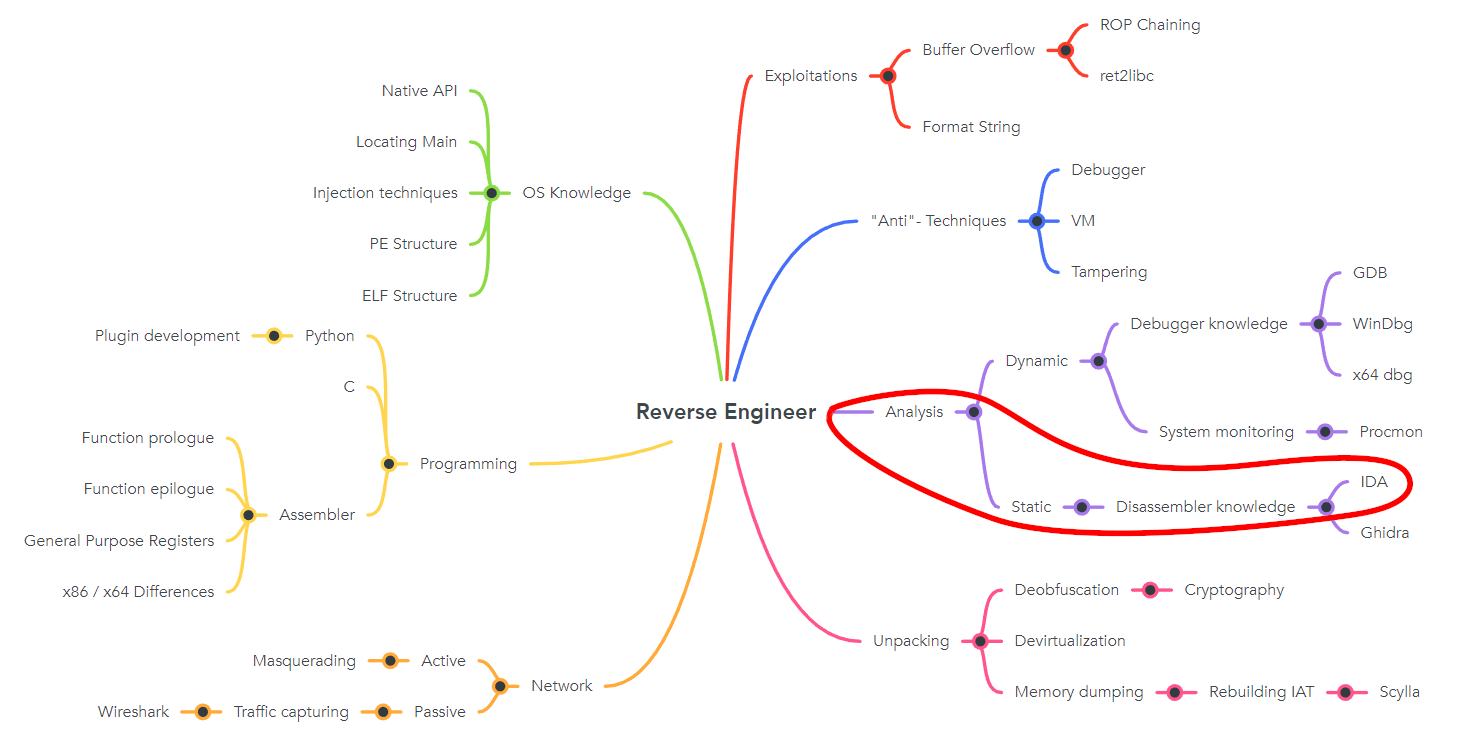
\includegraphics[width=\textwidth]{resources/IDAIntro-overview-light.png}
    \caption{IDAIntro domain overview}
    \label{fig:IDAIntro-overview}
\end{figure}
\subsubsection*{Content}
This introduction explains all the relevant functionalities of IDA and how to install it.
\subsubsection*{Choice of Topic}
Some of the Reverse Engineers most powerful tools are disassemblers. We purposely chose IDA Freeware over Ghidra for the beginning. This prevents the students from just generating pseudo code instead of actually reading and understanding the assembly instructions in later labs. Because of this, the solutions of future labs are presented using IDA Freeware.
\subsubsection*{Objectives}
\begin{itemize}
    \item Install IDA Freeware and get a brief overview
    \item Learn to orient yourself in IDA and get ready to use it on a binary.
\end{itemize}
\subsubsection*{Grading}
The introduction labs are not graded since they are only used as a lookup. They have a flag to make sure the students have read the tools.
\pagebreak
% ------------------------------------------ LABS ------------------------------------------ %

\subsection{Lab 1: Asm-Refresher}
\subsubsection*{Problem Domain}
This lab covers the following aspects of the reverse engineering problem domain created by us:
\vspace{-2ex}
\begin{figure}[H]
    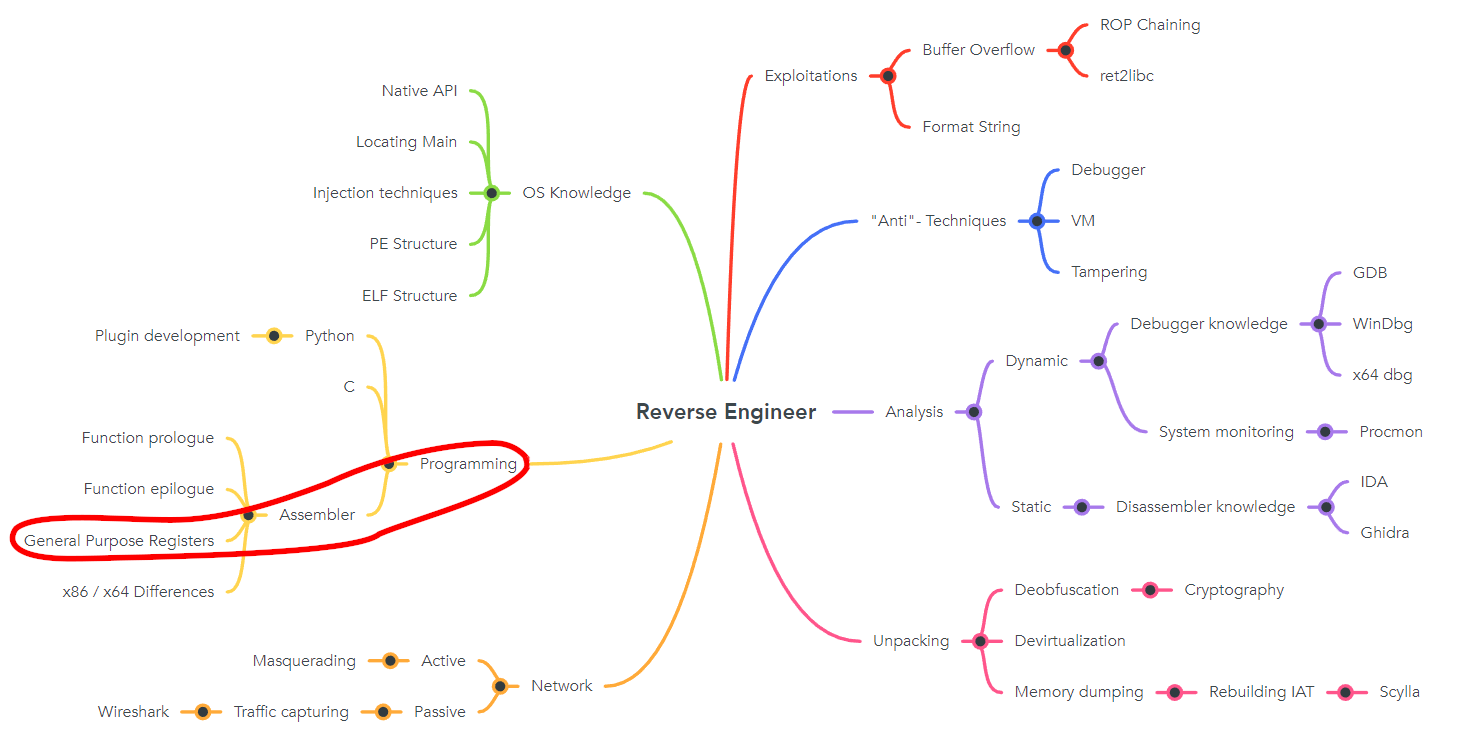
\includegraphics[width=\textwidth]{resources/ASM-overview-light.png}
    \caption{ASM refresher domain overview}
    \label{fig:refresher-overview}
\end{figure}
\subsubsection*{Content}
This lab is designed to be a refresher for those who have not done anything assembly related in a while. It covers the basic assembly instructions, explains the General-Purpose Registers and rounds up with a guide on how to write a "Hello World" program.  
\subsubsection*{Choice of Topic}
A reverse engineer has to understand the basic concepts of assembly. Not only when reading through dissasembled code but also later on when automatic pseudo code generation fails.
\subsubsection*{Objectives}
\begin{itemize}
    \item Refresh knowledge about the general-purpose registers.
    \item Basic understanding of assembly instructions
\end{itemize}
\subsubsection*{Grading}
This lab will not be graded since it is meant to help the students in later labs if they struggle with assembly.
\pagebreak

\subsection{Lab 2: Static Debugging}
\subsubsection*{Problem Domain}
This lab covers the following aspects of the reverse engineering problem domain created by us:
\vspace{-2ex}
\begin{figure}[H]
    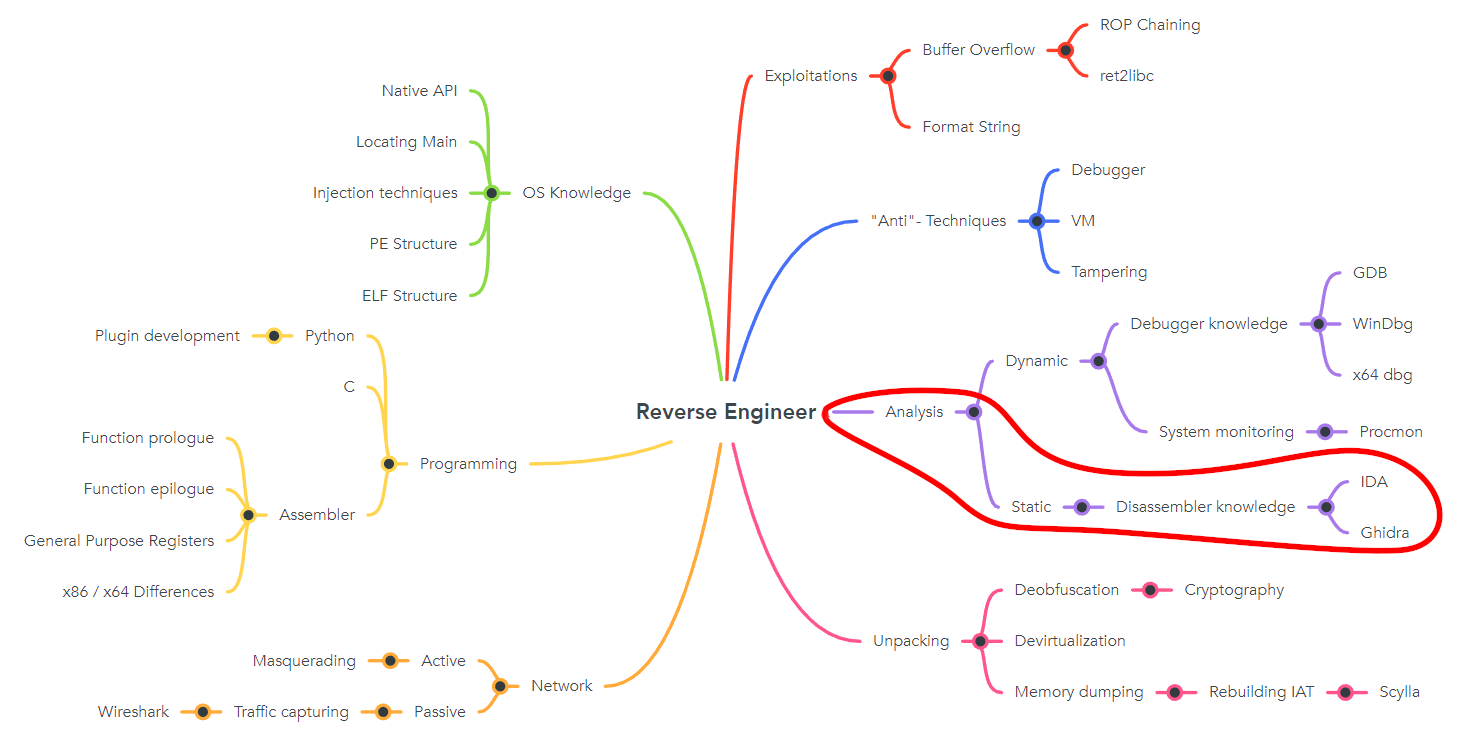
\includegraphics[width=\textwidth]{resources/static-overview-light.png}
    \caption{Static debugging domain overview}
    \label{fig:static-overview}
\end{figure}
\subsubsection*{Content}
In this lab the student will learn how to use IDA Freeware to statically reverse a given binary. The goal is to find the main function in a binary with and one without symbols. \\
This will show the student that seemingly simple things such as finding the main function can be a real problem if you have insufficient knowledge of the inner workings of a binary and the automatic detection of IDA fails.
\subsubsection*{Choice of Topic}
Program execution starts from the main() function which is why it is an important skill of a reverse engineer to find it and start understanding the rest of the binary from there on.
\subsubsection*{Objectives}
\begin{itemize}
    \item Find the main function in a normal binary
    \item Find the main function in a binary with symbols stripped
\end{itemize}
\subsubsection*{Grading}
The student has to inspect the main functions and find a flag in both of them. The final hand-in will be the combined flag.
\pagebreak

\subsection{Lab 3: Dynamic Debugging}
\subsubsection*{Problem Domain}
This lab covers the following aspects of the reverse engineering problem domain created by us:
\vspace{-2ex}
\begin{figure}[H]
    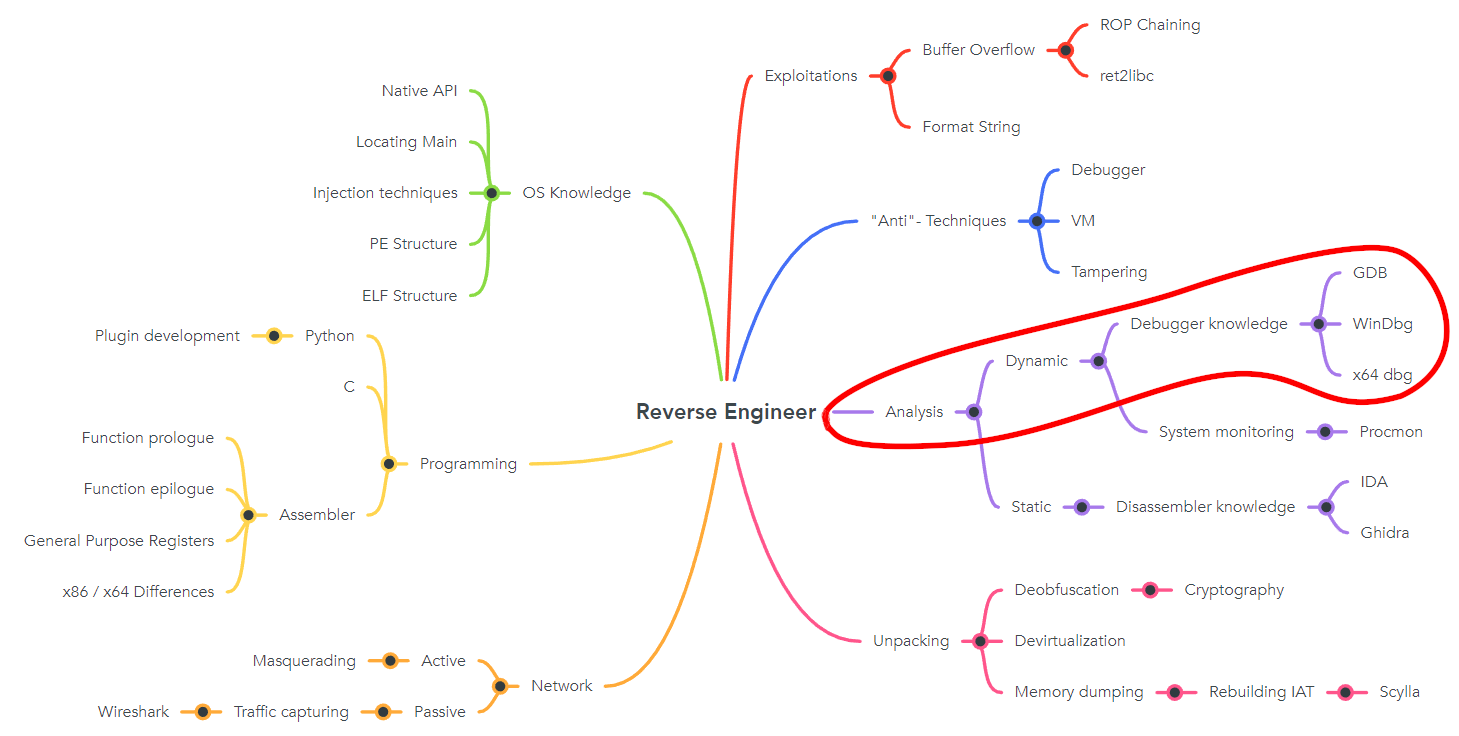
\includegraphics[width=\textwidth]{resources/dynamic-overview-light.png}
    \caption{Dynamic debugging domain overview}
    \label{fig:dynamic-overview}
\end{figure}
\subsubsection*{Content}
In this lab the student will learn how to use GDB and x64dbg to dynamically reverse a given binary. In a first step the lab explains how to dynamically debug the binary given in lab 2 and then, in a second step, the student will be presented with a new binary containing a flag. \\
The goal of this lab is to show the student how this skill is used and then have him do it on his own to solidify the steps he has completed before.
\subsubsection*{Choice of Topic}
Next to static debugging, dynamic debugging is used in a wide range of reverse engineering. Because of this it is important to have a student go through the steps and explain how it is done. 
\subsubsection*{Objectives}
\begin{itemize}
    \item Use GDB or x64dbg to find the flag of the binary
    \item Find the flag of a new binary using dynamic debugging
\end{itemize}
\subsubsection*{Grading}
The student has to use the newly aquired skills to find the flag in a new binary using dynamic debugging skills.
\pagebreak

\subsection{Lab 4: First Reversing Attempts}
\subsubsection*{Problem Domain}
This lab covers the following aspects of the reverse engineering problem domain created by us:
\vspace{-2ex}
\begin{figure}[H]
    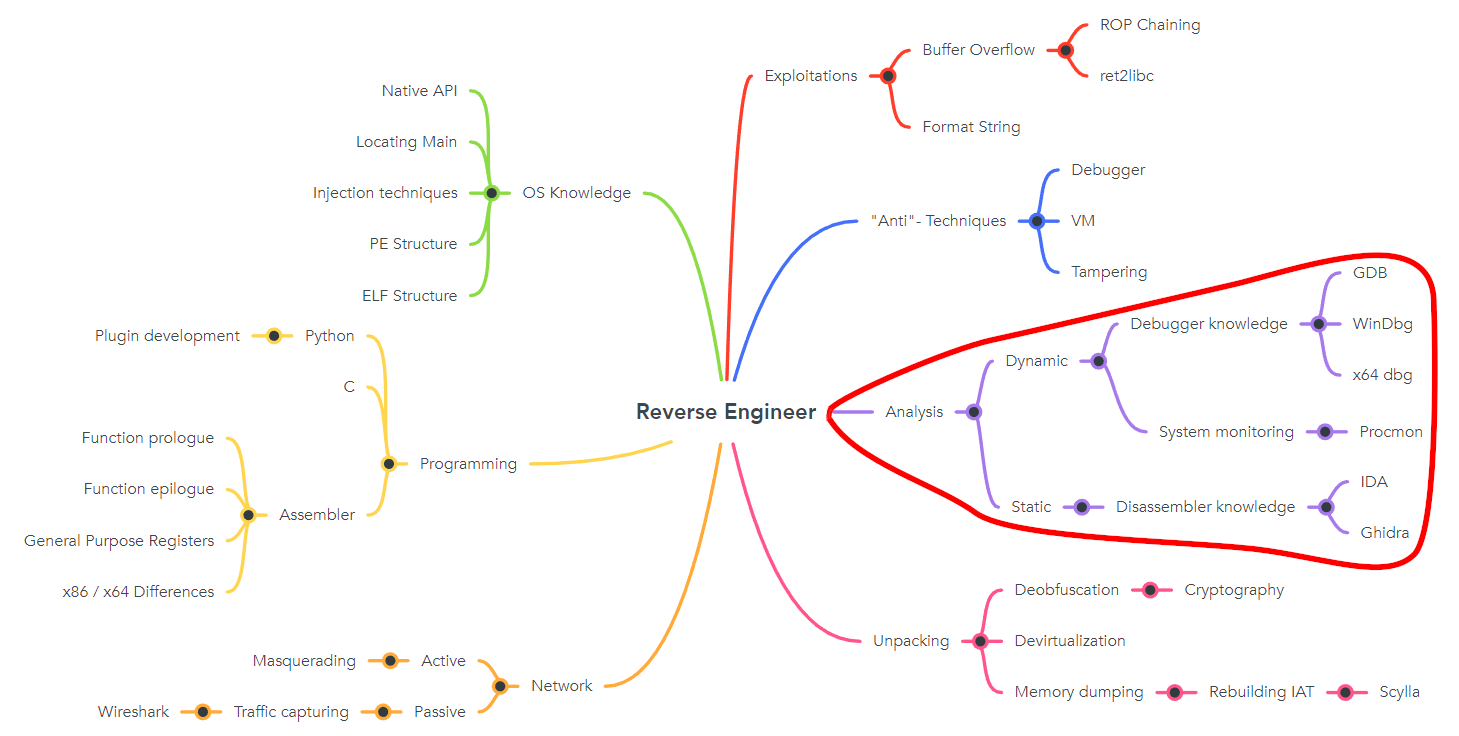
\includegraphics[width=\textwidth]{resources/reattempts-overview-light.png}
    \caption{RE attempts domain overview}
    \label{fig:reattempts-overview}
\end{figure}
\subsubsection*{Content}
In this lab the student will deepen his knowledge of reversing binaries to find out how they work. This challenge contains two binaries having different requirements that have to be met in order for the student to receive the flags.
\subsubsection*{Choice of Topic}
It is important to give the students simple examples where they can play around and learn by doing without providing a step by step guide.
\subsubsection*{Objectives}
\begin{itemize}
    \item Use static or dynamic debugging to find the requirements of the programs
    \item Find out how program arguments are handled in assembly
\end{itemize}
\subsubsection*{Grading}
The student has to solve both binaries to get a flag.
\pagebreak

\subsection{Lab 5: Remote Login}
\subsubsection*{Problem Domain}
This lab covers the following aspects of the reverse engineering problem domain created by us:
\vspace{-2ex}
\begin{figure}[H]
    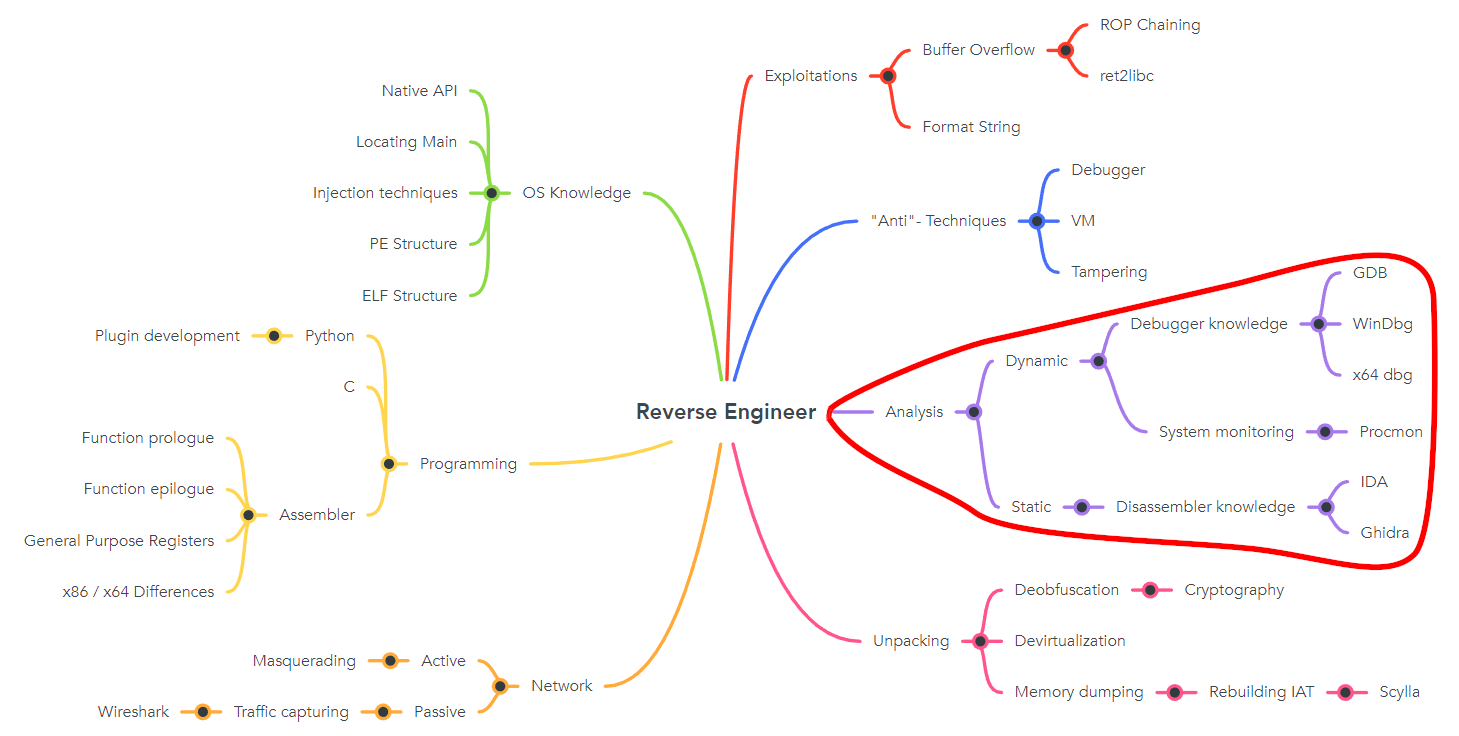
\includegraphics[width=\textwidth]{resources/remotelogin-overview-light.png}
    \caption{Remote login domain overview}
    \label{fig:remotelogin-overview}
\end{figure}
\subsubsection*{Content}
This lab dives deeper into the reverse engineering rabbit hole and introduces a new concept. The student first starts a docker container off a provided resource.
This docker container exposes a webserver and a port where an application runs. The application running on the server can be downloaded from the servers website by the student. \\
The student then has to combine dynamic and static reverse engineering to figure out the password in order to log into the server and expose the flag.
\subsubsection*{Choice of Topic}
Giving the students an idea that reverse engineering can be used to gather information that you can later exploit on a target system.
\subsubsection*{Objectives}
\begin{itemize}
    \item Learn to use the tools you got introduced to
    \item Apply basics of dynamic and static debugging and find a way to exploit remote target 
\end{itemize}
\subsubsection*{Grading}
The student has to find out the flag and submit a small writeup to answer the security questions provided.
\pagebreak

\subsection{Lab 6: Pwntools - Introduction}
\subsubsection*{Problem Domain}
This lab covers the following aspects of the reverse engineering problem domain created by us:
\vspace{-2ex}
\begin{figure}[H]
    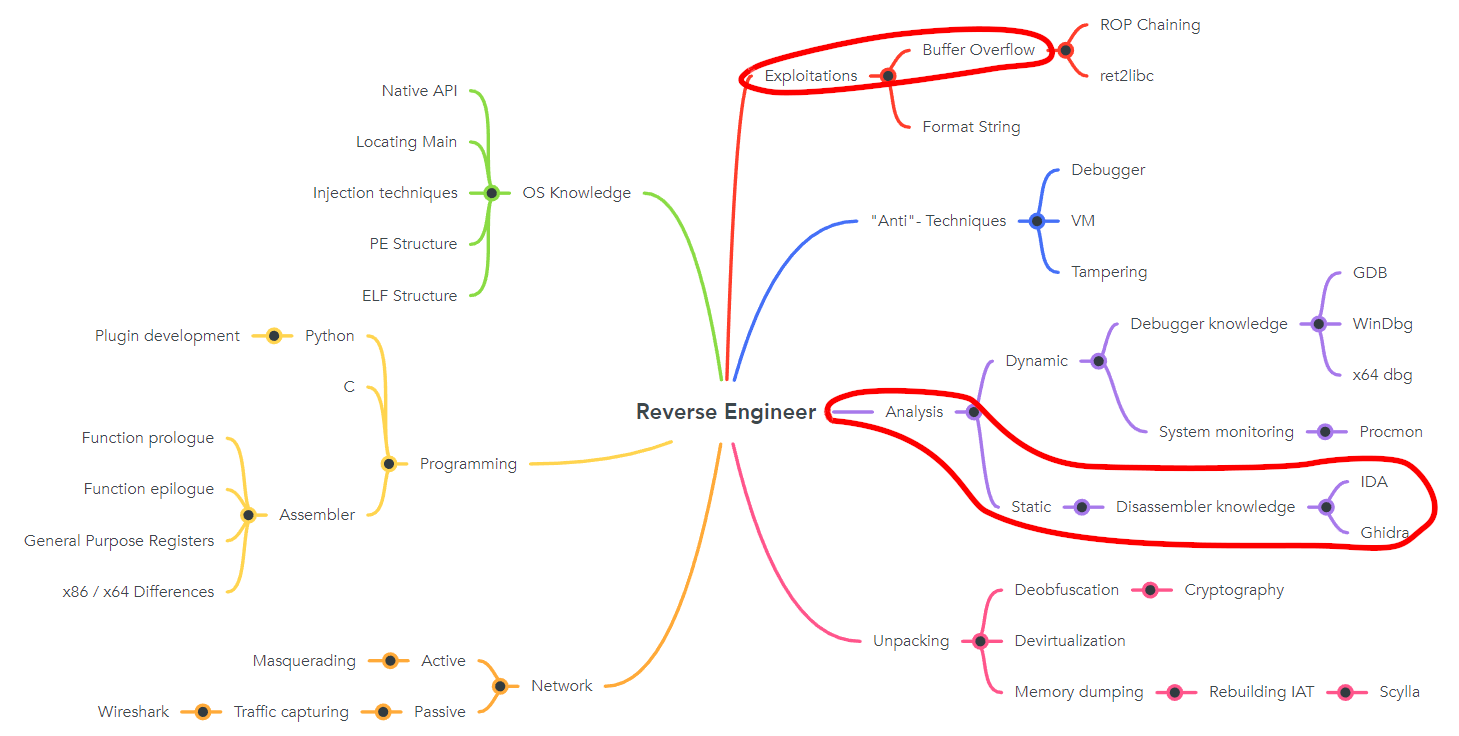
\includegraphics[width=\textwidth]{resources/pwntools-overview-light.png}
    \caption{Pwntools domain overview}
    \label{fig:pwntools-overview}
\end{figure}
\subsubsection*{Content}
In this lab the student has a first introduction into the pwntool module of python. The student first has to start a docker conatiner from the provided resource. This docker exposes both a webserver and a port where the application is running on. The student then downloads the compiled application to analyze it and search for a weakness to exploit. This weakness can then be exploited through the use of pwntools. Since this is a first introduction, the whole process of creating the script is guided as a walkthrough.
\subsubsection*{Choice of Topic}
Pwntools is an important module to learn for exploiting. Reverse engineering in general is widely used to find vulnerabilities to exploit, which means it is important for a student to not only know how to find the weakness but also how to exploit it.
\subsubsection*{Objectives}
\begin{itemize}
    \item Use acquired skills to find vulnerability in binary
    \item Create a pwntools script to exploit that vulnerabilty
\end{itemize}
\subsubsection*{Grading}
The grading is done by sending in the printed out flag when the script is run on the exposed port and a writeup answering the provided security questions.
\pagebreak

\subsection{Lab 7: Crypto Lab - AES ECB}
\subsubsection*{Problem Domain}
This lab covers the following aspects of the reverse engineering problem domain created by us:
\vspace{-2ex}
\begin{figure}[H]
    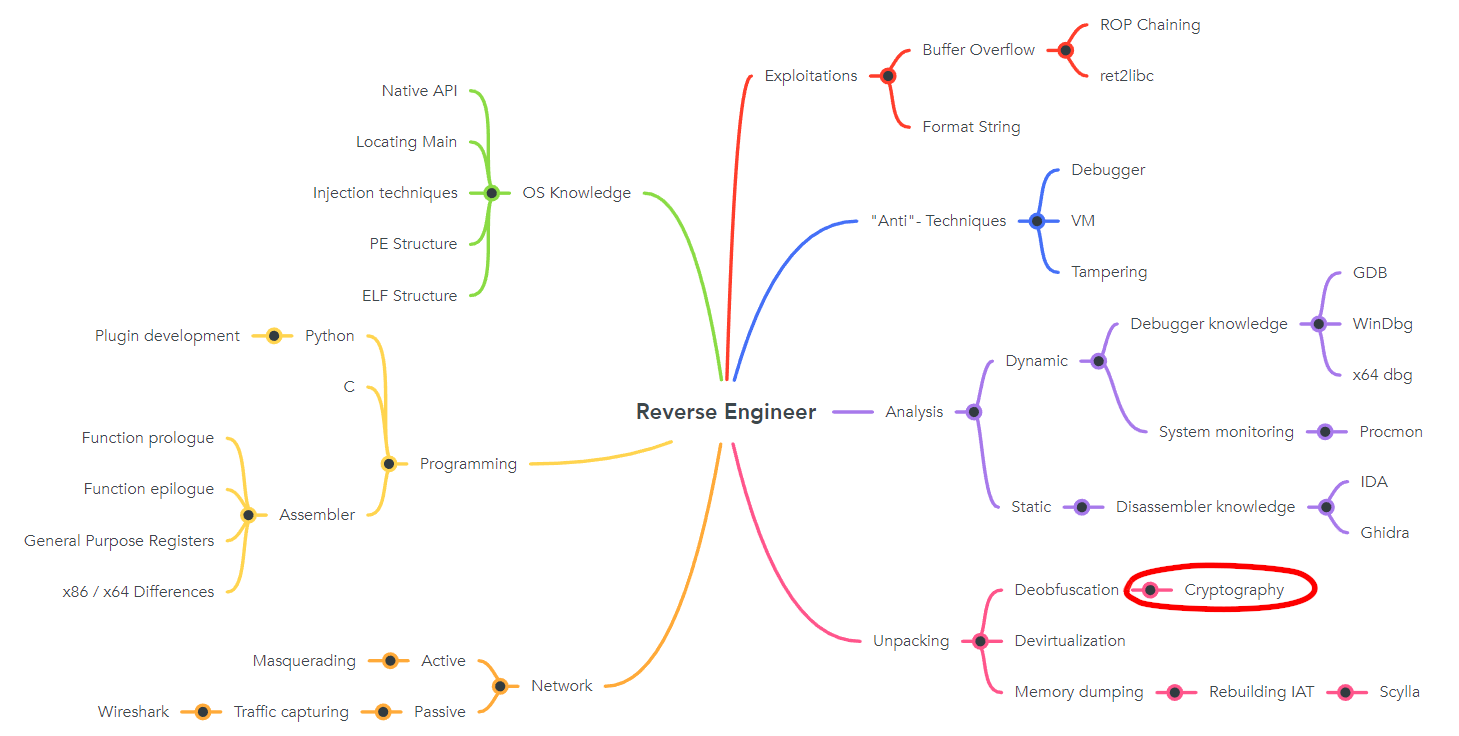
\includegraphics[width=\textwidth]{resources/aes-overview-light.png}
    \caption{AES domain overview}
    \label{fig:aes-overview}
\end{figure}
\subsubsection*{Content}
The student is presented a docker container which runs a webserver and exposes a port on which the script for the student to crack is running. The student first inspects and analyzes the script itself and then follows a walkthrough on how to write a simple script which exploits a common vulnerability in AES ECB mode. 
\subsubsection*{Choice of Topic}
Encryption is a widely used form of obfuscation. Because of this it is important as a cyber security student to be informed about certain weaknesses these ciphers have and how to exploit them if needed. 
\subsubsection*{Objectives}
\begin{itemize}
    \item Find out how the script works
    \item Find patterns to exploit
    \item Create a pwntools script to crack the encryption
\end{itemize}
\subsubsection*{Grading}
The grading is done by sending in the printed out flag when the script is run on the exposed port in combination with a writeup answering the provided security questions.
\pagebreak

\subsection{Lab 8: Patching Lab}
\subsubsection*{Problem Domain}
This lab covers the following aspects of the reverse engineering problem domain created by us:
\vspace{-2ex}
\begin{figure}[H]
    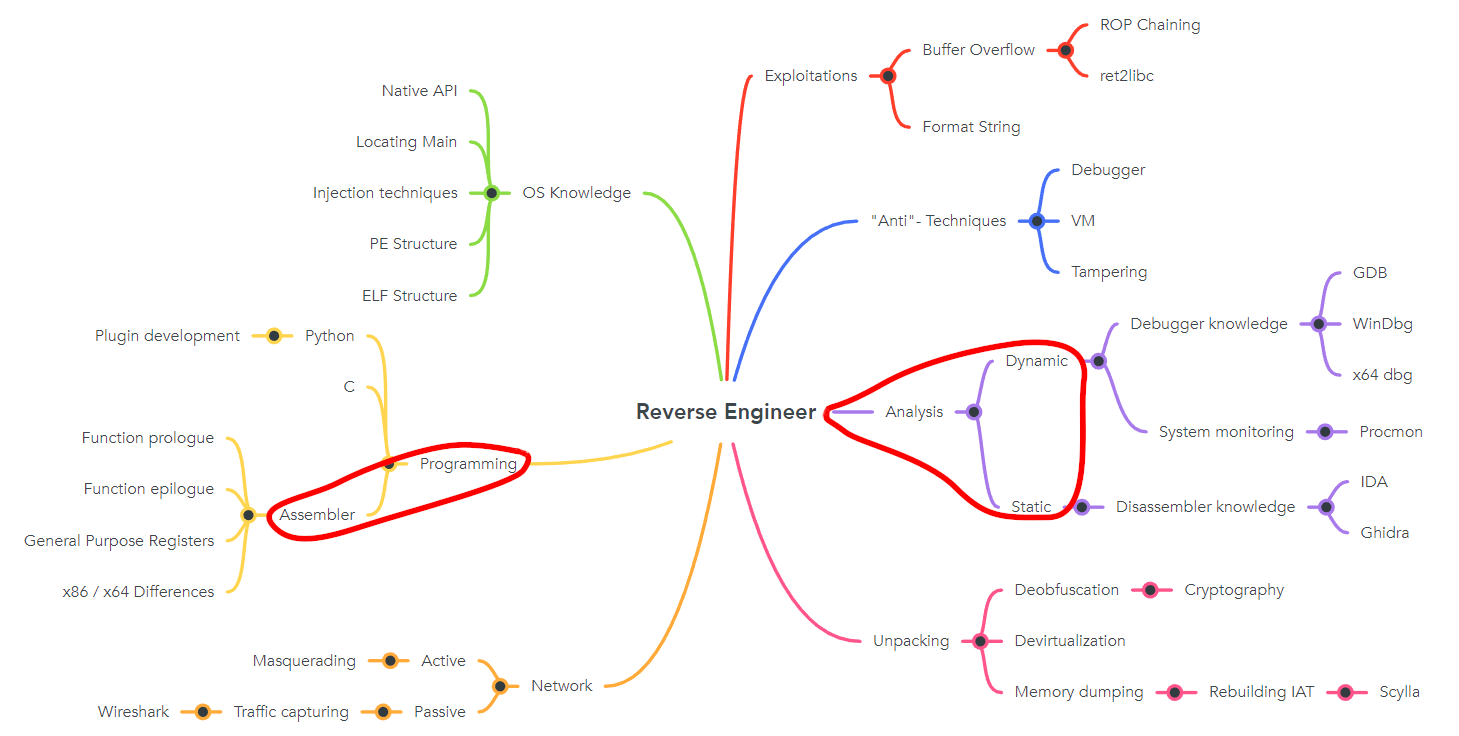
\includegraphics[width=\textwidth]{resources/patching-overview-light.png}
    \caption{Patching domain overview}
    \label{fig:patching-overview}
\end{figure}
\subsubsection*{Content}
The student is presented a binary which does not operate correctly. The student is tasked to find the location to patch and fix it. In order to check the patch generated by the user, the provided docker container starts up a webserver where the student can upload the patch file. The webserver then tries to apply the patch to a local copy of the binary and checks if the bug is fixed. If fixed, the webserver shows the flag to the student. If not fixed, the student has the possibility to reset the binary and try again.

\subsubsection*{Choice of Topic}
Reverse engineering also comes in handy when encountering bugs in software where the source code is unreachable. Therefore it is important to locate found bugs in an executable and know how to apply patches.
\subsubsection*{Objectives}
\begin{itemize}
    \item Find the mistake of the binary
    \item Change the ASM code and upload the patched file to the website
\end{itemize}
\subsubsection*{Grading}
The grading will be done via a writeup and a flag.
\pagebreak


% --------------------------------------%
\section{Risk Analysis}
\chapter{Risks}
\section{Risk Managment}
For this project, the ”Project Management Triangle” is lacking the cost dimension, while the time dimension is fixed (strict deadlines). As a result, any risks that appear, automatically lead to a reduction of the project scope if there is no spare time. Because of this, we will prioritize dealing with risks above regular tasks and prioritize essential tasks over nice-to-haves, but we do not intend on planning in a flat time margin as we have no way to negotiate for more time.

\section{Estimated Risks}

\subparagraph{General Risks}
\begin{itemize}
    \item Finding Testing Participants (severity: medium, probability: high)\\ 
    \textbf{Mitigations:} Early looking for backup person \\ 
    \textbf{Actions taken:} Found backup person\\ 
    \textbf{New probability:} low
    \item Being able to create reverseable Programs with additional difficulties. (severity: very high, probability: medium)\\ 
    \textbf{Mitigations:} being able to ask Ivan \\ 
    \textbf{Actions taken:} Asked for possible help\\ 
    \textbf{New probability:} low
    \item Irreparable corruption of git server. (severity: very high, probability: low)\\ 
    \textbf{Mitigations:} Weekly off-site git server backups\\
    \textbf{Actions taken:} Repository mirrored to GitHub\\ 
    \textbf{New severity:} low
    \item Irreparable corruption of git server. (severity: very high, probability: low)\\ 
    \textbf{Mitigations:} Weekly off-site git server backups\\
    \textbf{Actions taken:} Repository mirrored to GitHub\\ 
    \textbf{New severity:} low
    \item Lost work due to un-pushed work. (severity: low, probability: high)\\ 
    \textbf{Mitigations:} Frequent reminders to push changes by Scrum Master / Team\\
\end{itemize}
\subparagraph{License Complications}
\begin{itemize}
    \item License Problems with Ghidra. (severity: high, probability: very low)\\ 
    \textbf{Mitigations:} No mitigations needed because it's completely Open Source.
    \item License Problems with IDA. (severity: high, probability: low)\\ 
    \textbf{Mitigations:} Providing a previously free version
\end{itemize}
